
\section{Introduction}

In this chapter we will discuss about our research findings and will compare it to the existing method. In this study we tried to detect vehicles from a mixed dataset which contained 21 vehicles from Bangladesh and India. We will show how our proposed methods perform compared to other well known methods and models and how it can be used in modern tasks.

\section{Result Metrics Analysis}
Here is the definition of the result metrics we are finding from our study.
\subsection{Classification} 
In machine learning, classification refers to a predictive modeling problem where a class label is predicted for a given example of input data. 
Classification measured with confidence score  also known as accuracy or precision which is defined in percentage(\%) or between 0 to 1. We used both measuring method in our study. The equation for calculating precision score is:

\begin{equation}
    precision = \frac{True \ Positive}{True \ Positive+False \ Positive}
\end{equation}

\begin{table}[!h]
  \centering
  \caption[Evaluation of the Model]{Evaluation of the model on the validation set with an IoU threshold of 45\% that is the 
Area-Under-Curve for each unique Recall. }
  \label{tab:class-ap}
  {\renewcommand{\arraystretch}{1.1}
    \begin{tabular}{p{4.3cm} p{1cm} p{1cm} p{1cm} p{1cm} p{1cm}}
          \toprule
          Class/Epoch                       & 3 (\%) & 6 (\%) & 9 (\%) & 12(\%)  & 15(\%) \\
          \hline
          Ambulance                   & 00.27    &  00.89 & 01.04  & 01.67   & 02.05  \\
          Auto Rickshaw               & 01.16    &  02.41 & 05.96  & 08.15   & 08.69  \\
          Bicycle                     & 03.01    &  03.87 & 07.11  & 09.83   & 11.27  \\
          Bus                         & 07.25    &  20.59 & 65.26  & 81.26   & 89.28  \\
          Car                         & 09.57    &  23.72 & 59.05  & 85.11   & 94.60  \\
          Garbage Van                 & 00.03    &  00.15 & 01.09  & 01.53   & 01.87  \\
          Human Hauler                & 00.75    &  01.04 & 03.43  & 07.29   & 06.49  \\
          Minibus                     & 01.03    &  01.97 & 05.18  & 06.34   & 07.20  \\
          Minivan                     & 06.30    &  08.29 & 19.07  & 29.47   & 37.91  \\
          Motorbike                   & 05.21    &  13.62 & 21.46  & 50.37   & 69.33  \\
          Pickup                      & 04.38    &  12.45 & 14.53  & 36.76   & 53.34  \\
          Army Vehicle                & 00.06    &  00.14 & 00.12  & 00.21   & 00.88  \\
          Police Car                  & 00.03    &  00.87 & 00.64  & 00.87   & 01.02  \\
          Rickshaw                    & 04.77    &  19.43 & 32.45  & 65.03   & 82.11  \\
          Scooter                     & 00.65    &  01.11 & 01.94  & 02.14   & 02.45  \\
          SUV                         & 03.86    &  12.32 & 23.76  & 32.54   & 41.34  \\
          Taxi                        & 00.43    &  01.54 & 02.86  & 03.95   & 04.44  \\
          Three Wheelers (CNG)        & 01.54    &  17.25 & 36.24  & 57.23   & 87.26  \\
          Truck                       & 05.49    &  16.38 & 31.86  & 56.67   & 76.63  \\
          Van                         & 03.76    &  13.74 & 27.97  & 43.17   & 53.91  \\
          Wheelbarrow                 & 01.49    &  09.32 & 15.34  & 22.39   & 23.29  \\
          \bottomrule
    \end{tabular}
  }
\end{table}



In our dataset there are 21 classes and we have a very high accuracy rate but the detection rate is low because of low data and ground truth bounding boxes. In~\ref{tab:vehicle_count} we can see classification accuracy for 6 classes: car, rickshaw, bus, SUV and truck. We can see the accuracy is gradually increasing but both wheelbarrow and SUV have very low accuracy compared to other 4 classes. This is because of very low data related to these 2 classes. We identified that there are a total 10 classes which have very low data compared to other 11 classes. 


\subsection{Counting} Counting in machine learning means how many same objects are in the predicted data. Though It is the sub product of classification, it can be used in many useful tasks. Like counting how many cars are passing by everyday and how many buses and trucks are there. The calculation of counting is simple. For this we need to calculate the classification result and store it as data so that we can use it later.

\begin{figure}[h]
    \centering
    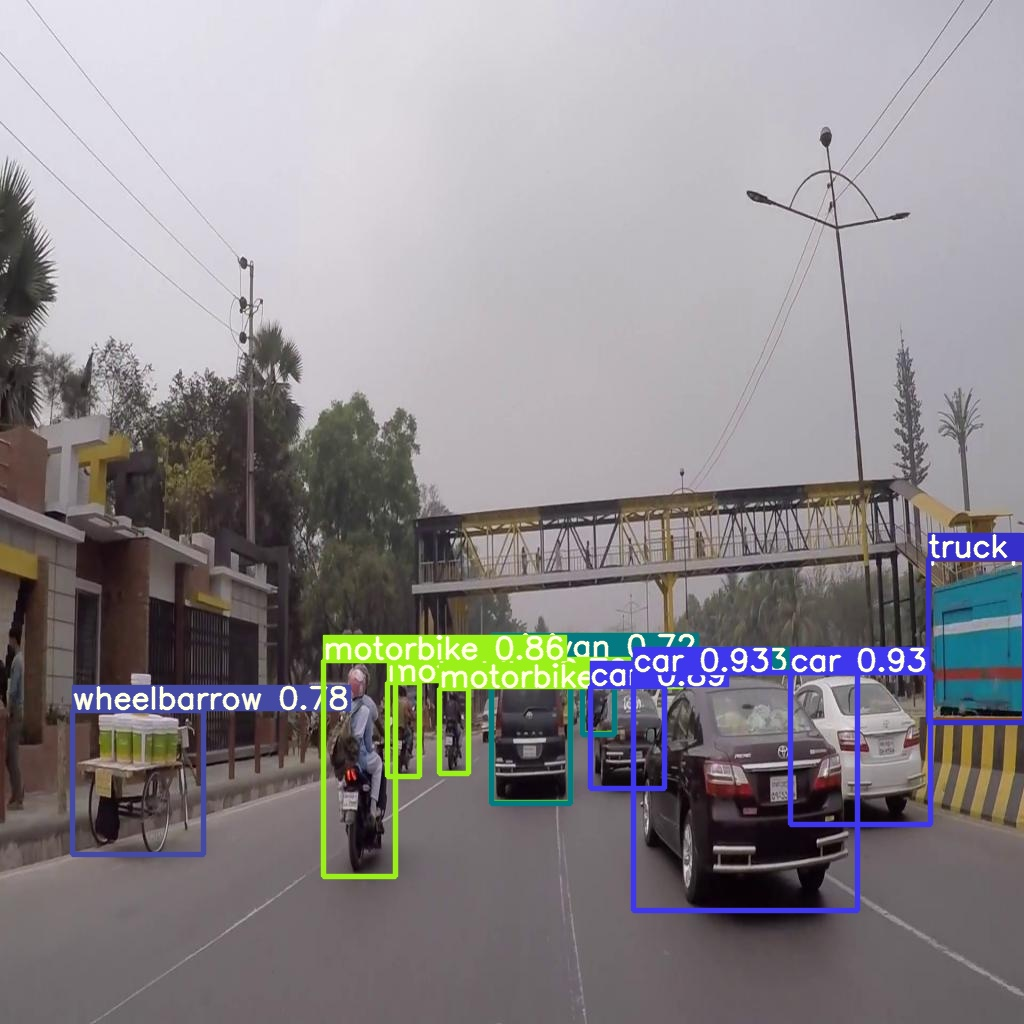
\includegraphics[max width=\textwidth]{images/ours/Asraf_51_jpg.rf.0e3516baf7509bc2c4a4aa8deea494c2.jpg}
   \caption[Inference Sample]{ Inference from the model of our proposed architecture}
    \label{fig:inference23}
\end{figure}

\begin{table}[!h]
  \centering
  \caption[Vehicle Count]{Vehicle count}
  \label{tab:vehicle_count}
  {\renewcommand{\arraystretch}{1.1}
    \begin{tabular}{p{2cm} p{3cm} p{3cm}}
          \toprule
            Class ID & Class Name & Class count \\
          \hline
            5 & car & 3 \\
            9 & minival & 2 \\
            10 & motorbike & 3 \\
            19 & truk & 1 \\
            21 & wheelbarrow & 1 \\
          \bottomrule
    \end{tabular}
  }
\end{table}

In~\ref{tab:vehicle_count} we showing counting of vehicles from~\ref{fig:inference23}.



\subsection{Detection} Detection known as Image Localization, Image Localization will specify the location of single object in an image whereas Object Detection specifies the location of multiple objects in the image. 
Detection mostly use bounding box to detect object from image. Bounding box is a rectangle. The measuring method for detection is mAP(mean average precision) which is calculated by :  


\begin{equation}
  mAP =\frac{1}{n} \displaystyle\sum\limits_{i=0}^n\frac{True \  Positive \ \tiny i}{(True \ Positive + False \ Positive) \ \tiny i}
\label{eqn:mAP}
\end{equation}

\begin{figure}[h]
    \centering
    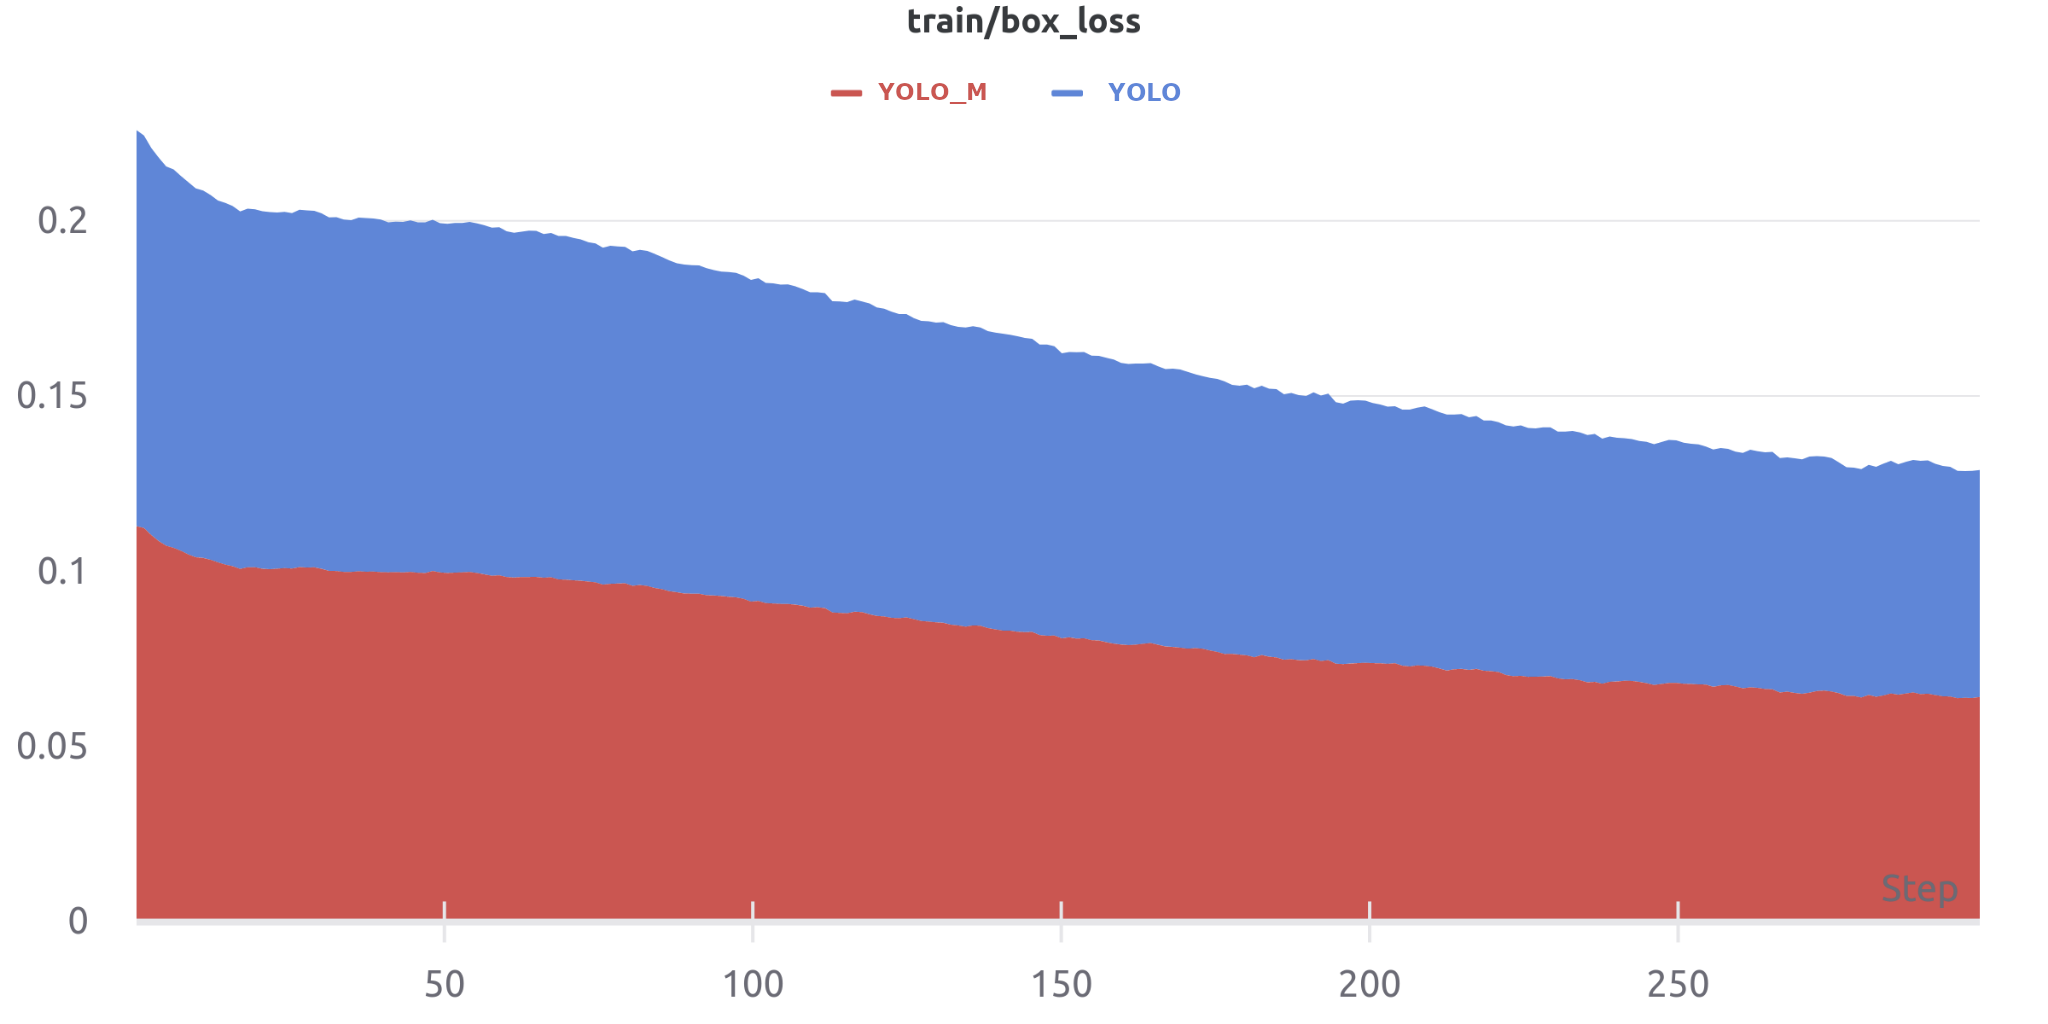
\includegraphics[max width=\textwidth]{images/ours/box-loss.png}
   \caption[Box Loss Comparison of Proposed Model and YOLOv5]{Bounding box loss comparison of our proposed model and YOLOv5}
    \label{fig:box_loss}
\end{figure}
\subsection{Comparison of Loss }
In~\ref{fig:box_loss} we can see comparison of detection box loss during training our model and YOLOv5 model. Loss is the penalty for a bad prediction. That is, loss is a number indicating how bad the model's prediction was on a single example. If the model's prediction is perfect, the loss is zero; otherwise, the loss is greater. The goal of training a model is to find a set of weights and biases that have low loss, on average, across all examples. Above blue is a loss for YOLOv5 model and red is a loss for your model. We can see that our model is almost 2x better compare to existing methods for detecting vehicles in our mixed dataset. We can see both model's loss is decreasing after each epoch but the initial difference is almost the same for all steps. By losing metrics we can see that our model is doing better.
\newpage
\begin{figure}[h]
    \centering
    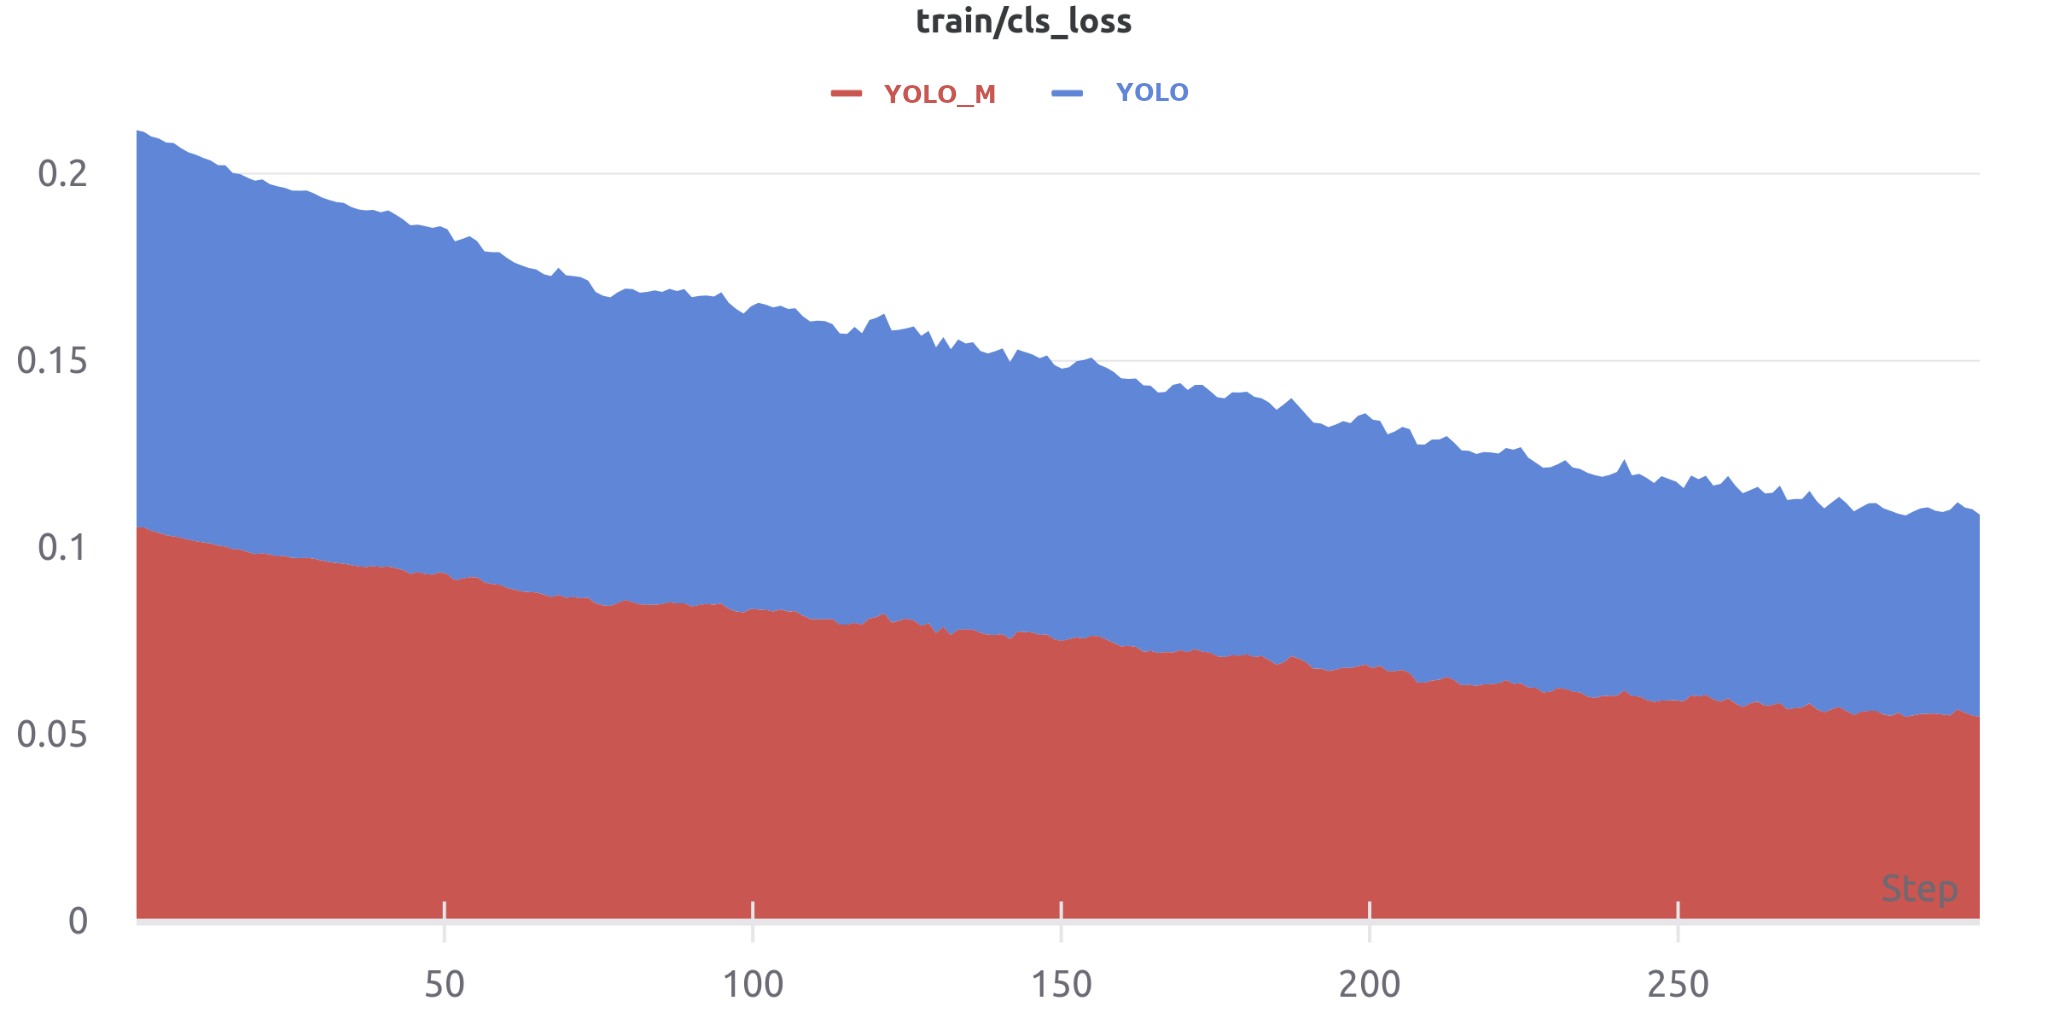
\includegraphics[max width=\textwidth]{images/ours/cls-loss.png}
   \caption[Classification Loss comparison of YOLOv5 and Our Proposed Model]{ Classification loss comparison of our proposed model and YOLOv5}
    \label{fig:cls_loss}
\end{figure}

In~\ref{fig:cls_loss} we can see classification loss comparison between YOLOv5 and our proposed method. We can see that both classification loss and box loss are almost identical because of YOLO's feature: it both detects and classifies objects at the same time. That is why it is known as “ you only look once” not like FasterRCNN or other models where we get different loss for classification and detection. Because those models use different methods for classification and detection inside the same model. So we can say our model beats YOLOv5 in both classification and detection loss. 

\subsection{Accuracy Comparison  }
This is the most important of any study. Here we will try to compare our model with the existing model and our parent model which we modified. 

\begin{figure}[h]
    \centering
    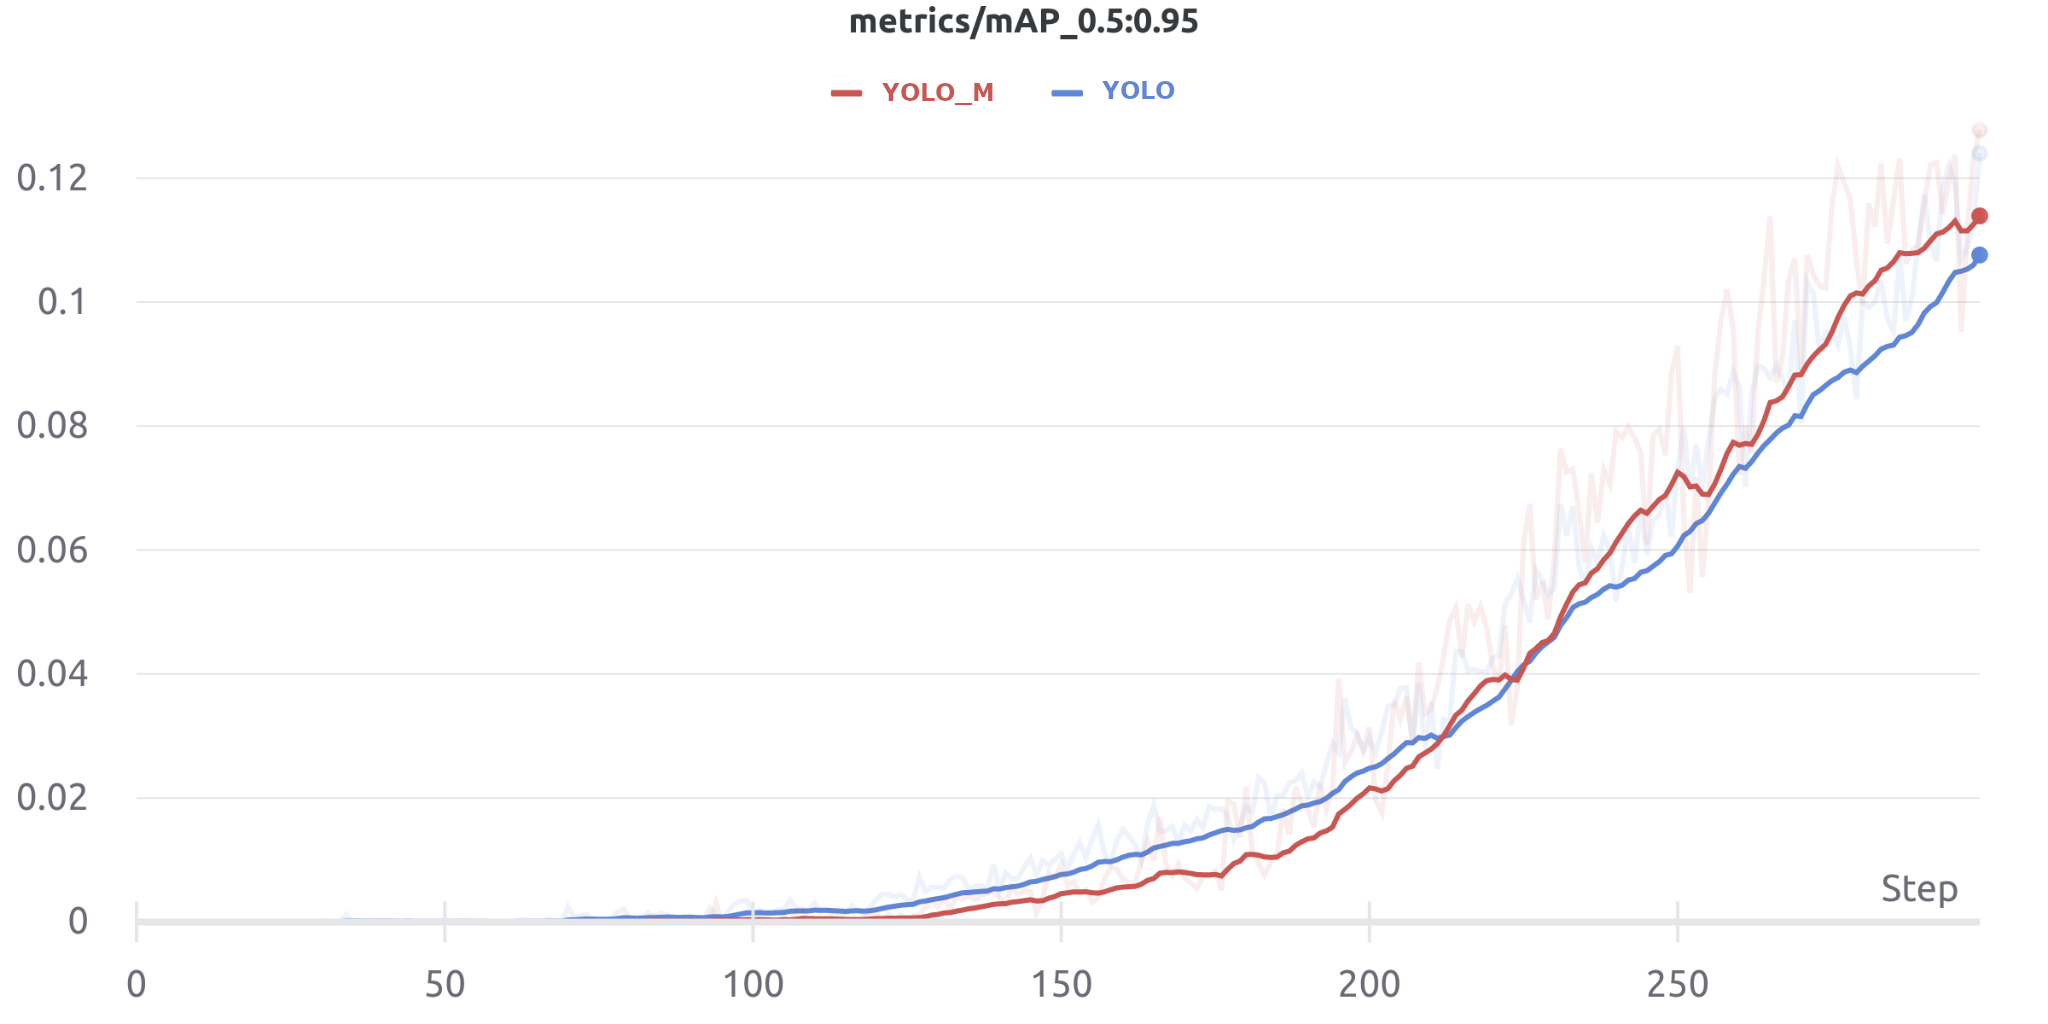
\includegraphics[max width=\textwidth]{images/ours/mAP.png}
   \caption[mAP Comparison of YOLOv5 and Our Proposed Model]{mAP comparison of YOLOv5 and our proposed model}
    \label{fig:mAP}
\end{figure}

In~\ref{fig:mAP} we can see our model mAP almost touch 0.13 during epoch 300 where YOLOv5 touches only 0.12. There is almost 0.1 (10\%) difference for our mixed Dhaka-Ai dataset. This result show that our model is doing better in both detection and classification. But the result of mAP is very low because of the less data in some classes. If we remove the class then the accuracy increases exponentially. But that will be researched in other studies. Currently we are studying 21 classes but only a few classes have enough data to be trained. We will be trying to reduce the classes so that we can improve our model for a few classes and use it in modern tasks. This model can easily detect bus, truck, car  without much effort but when it comes to classes which have low data like wheelbarrow, ambulance, garbage van etc it can not detect these classes very well. We have plan to study this dataset and model without the minor classes which has low data compared to others.

\begin{table}[!h]
  \centering
  \caption[Performance Comparison of Proposed Model with Various Models]{Performance comparison of proposed model with various models}
  \label{tab:model_comp}
  {\renewcommand{\arraystretch}{1.7}
      \begin{tabular}{p{4cm} p{1cm} p{0.8cm} p{1cm} p{2.6cm}}
          \toprule
          Model Name                                    & mAP (our dataset) & COCO mAP & Speed (ms) & Detect Small object and less overlapping \\
          \hline
          EfficientDet D4 1024x1024                     & 12.27             & 48.5     & 133        & YES                                      \\
          SSD ResNet152 V1 FPN 1024x1024 (RetinaNet152) & 8.75              & 38.3     & 104        & NO                                       \\
          Faster R-CNN ResNet101 V1 1024x1024           & 11.56             & 37.1     & 72         & NO                                       \\
          Faster R-CNN Inception ResNet V2 1024x1024    & 11.89             & 38.7     & 236        & NO                                       \\
          YOLO v5(1024x1024)                            & 12.06             & 49.7     & 65         & YES                                      \\
          YOLO v5(1024x1024) Modified (Proposed Method) & 13.46             & 49.8     & 70         & YES                                      \\
          \bottomrule
    \end{tabular}
  }
\end{table}

This is very unique dataset none research has been made with this dhaka-ai mixed dataset. For this we run it into many different models like EfficientDet D4, SSD ResNet152 V1 FPN , Faster R-CNN ResNet101 V1 , Faster R-CNN Inception ResNet V2 , YOLO v5. After training the 


\newpage
\section{Prediction Result Analysis}
In this section we will discuss about prediction results of our model.

\begin{figure}[h]
    \centering
    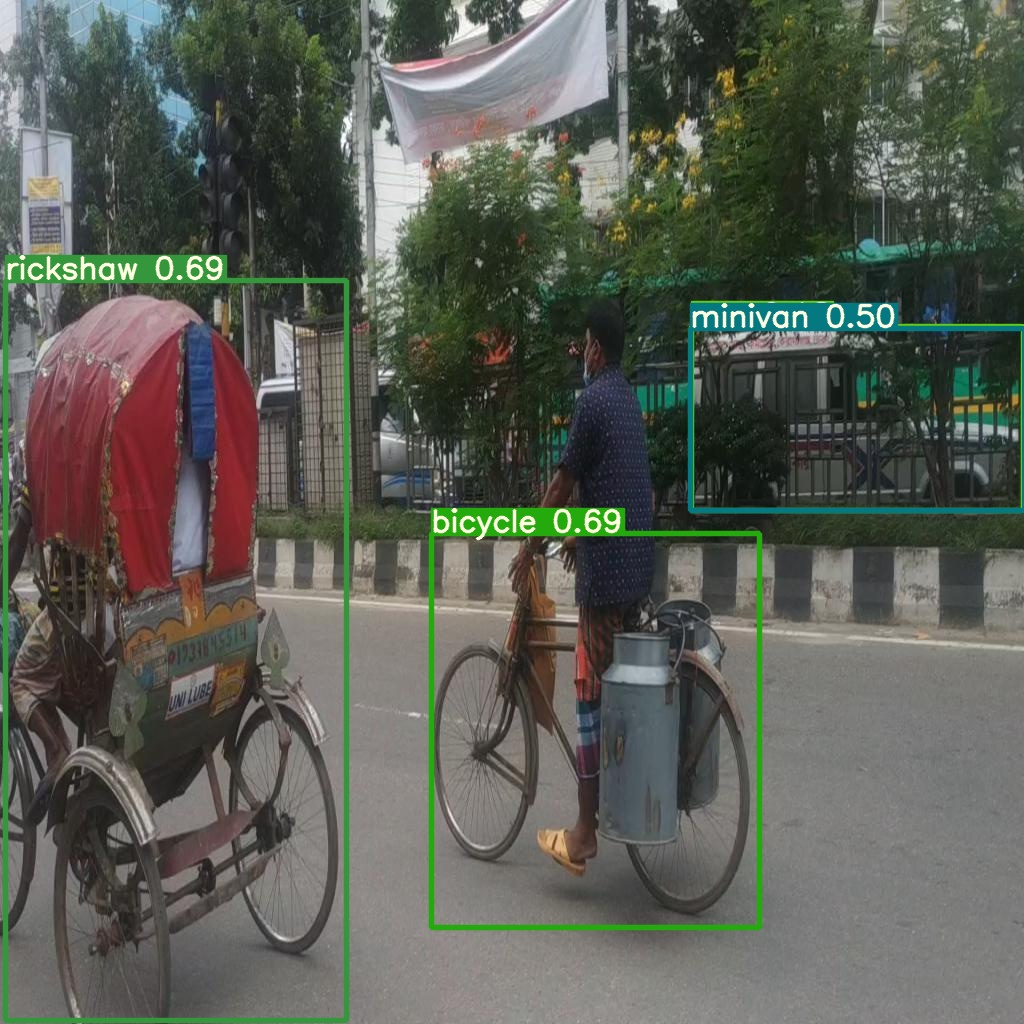
\includegraphics[max width=\textwidth]{images/ours/2.jpg}
   \caption[Sample Inference of Vehicles 1]{Sample inference of vehicles prediction near a road fence}
    \label{fig:inference345}
\end{figure}

\newpage
In~\ref{fig:inference345} we can see our model classified rickshaw and bicycle with confidence score 0.69 and minivan with 0.5 confidence score which is true positive and the bounding box is also in good shape. But if we look closely we can see this model can't detect other vehicles which is other side of the fence and have low visibility. Sometimes this kind of situation gives false positive results. 

\begin{figure}[h]
    \centering
    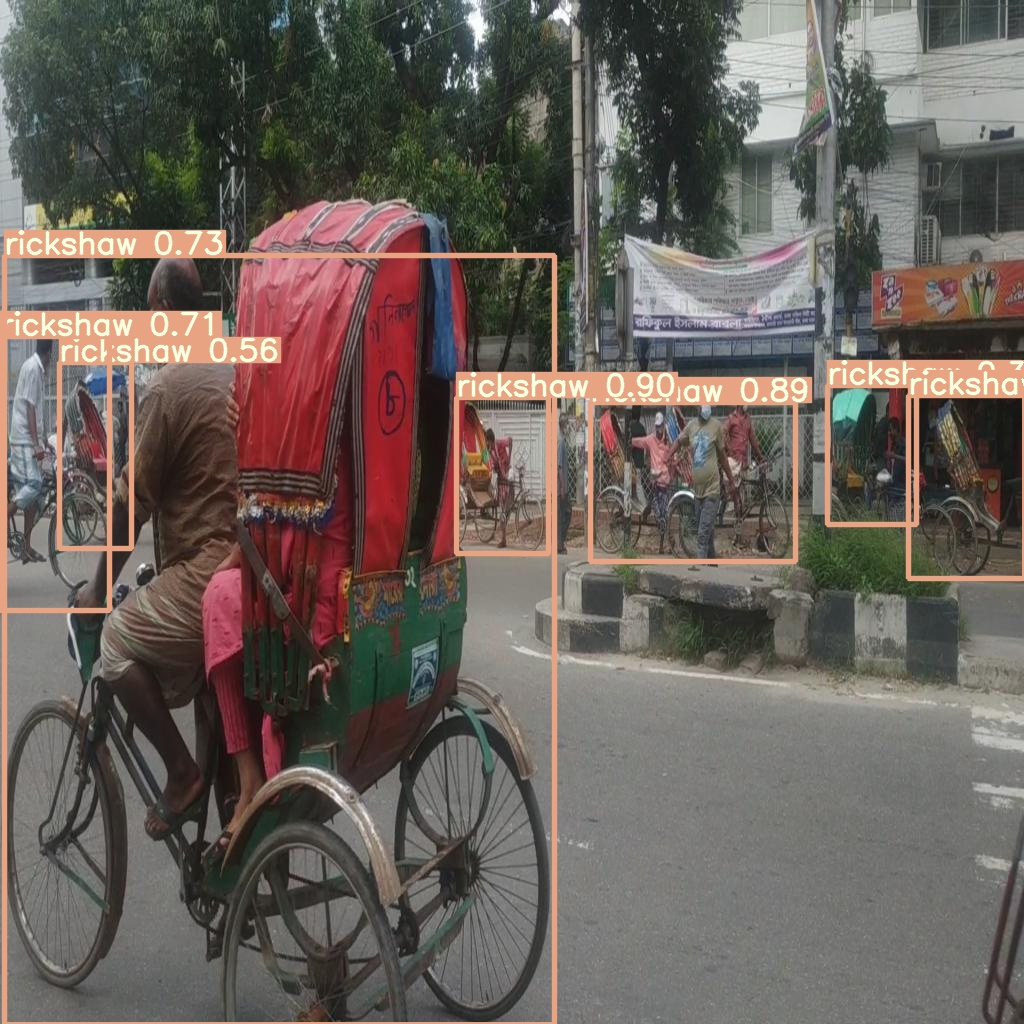
\includegraphics[max width=\textwidth]{images/ours/inference-2.jpg}
   \caption[Sample Inference of Vehicles 2]{Sample inference of multiple vehicles of same class}
    \label{fig:inference43}
\end{figure}

In~\ref{fig:inference43} we can see multiple vehicle of same class is there. We can see that it can easily identify rickshaws where confidence scores differ by the size of the vehicle. We can also see that sometimes two or more vehicles overlapped as one because of the IoU (intersection of union).

\newpage

\begin{figure}[h]
    \centering
    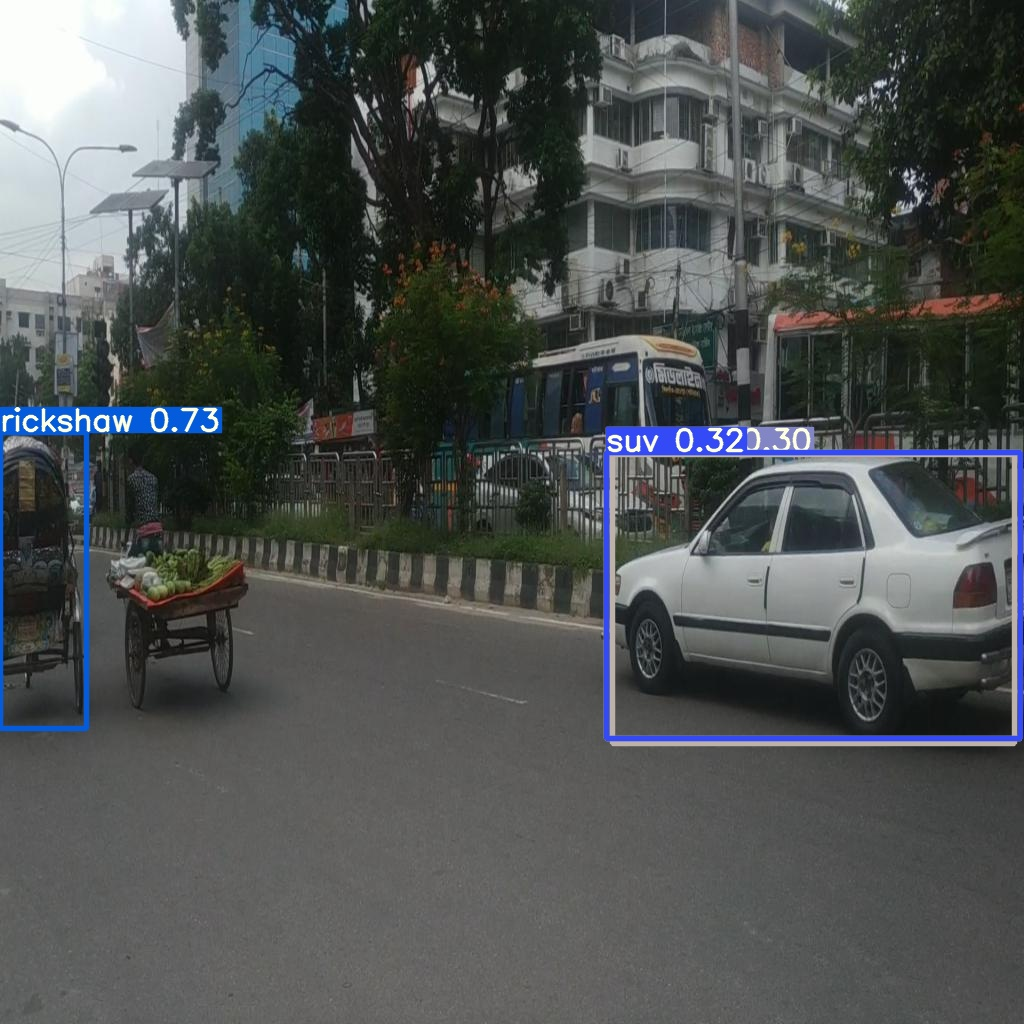
\includegraphics[max width=\textwidth]{images/ours/1.jpg}
   \caption[Sample Inference of Vehicles 3]{Sample inference of false positive and undetected vehicles}
    \label{fig:inference2354}
\end{figure}

In~\ref{fig:inference2354} we can see rickshaw is detected perfectly but the vehicle wheelbarrow and buses from other side of road fence is not detected. Because of the missing edges of the vehicles. Also we can see a false positive where our model detects the car as SUV with confidence score 0.32 and car as 0.30. It happens because of low data on SUV and wheelbarrow vehicles. 

\newpage

\begin{figure}[h]
    \centering
    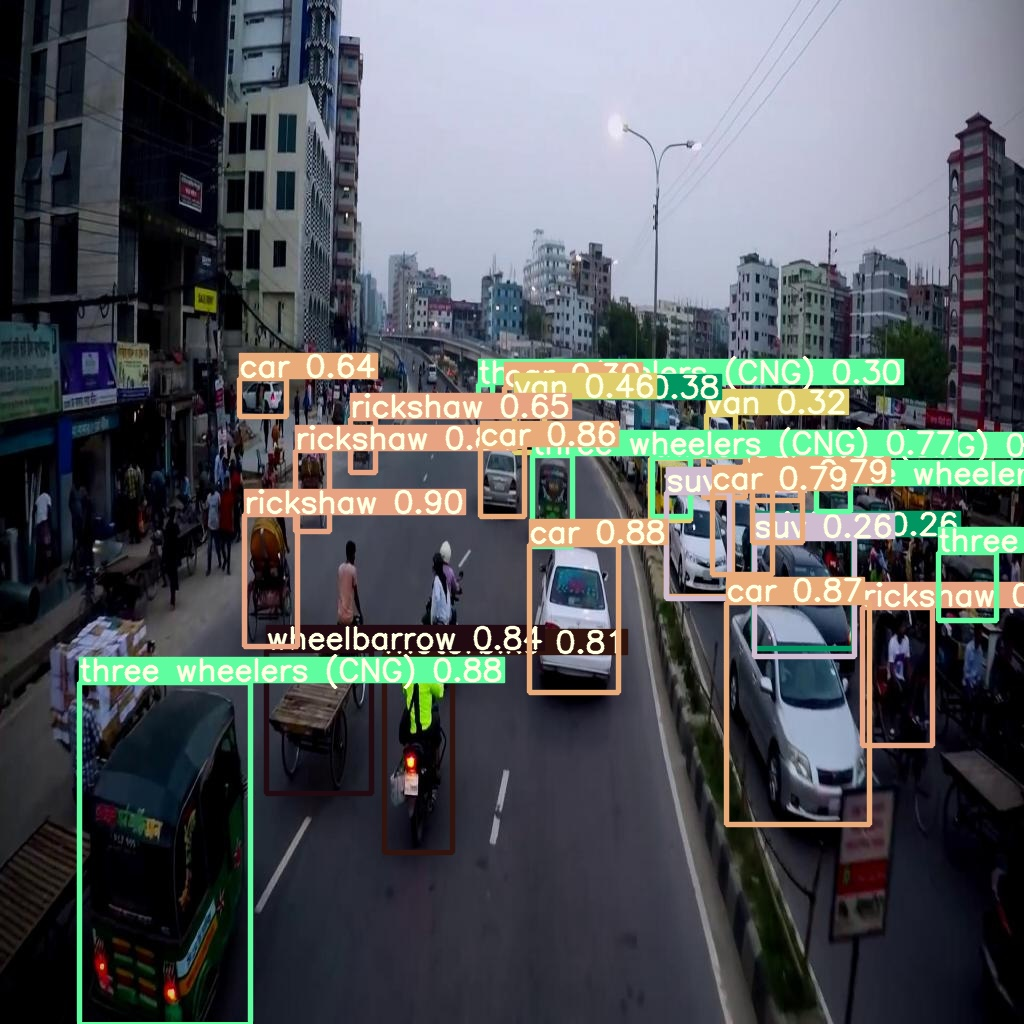
\includegraphics[max width=\textwidth]{images/ours/3 (2).jpg}
   \caption[Sample Inference of Vehicles 5]{ Sample inference of multiple types of vehicles}
    \label{fig:inference875}
\end{figure}

In~\ref{fig:inference875} we can see our model detecting multiple type of vehicles but missing some wheelbarrow. We can also see our model giving very low false positives and detecting vehicles in distance with a good confidence score. This image is in dusk but it is still predicating with good accuracy.

\newpage

\begin{figure}[h]
    \centering
    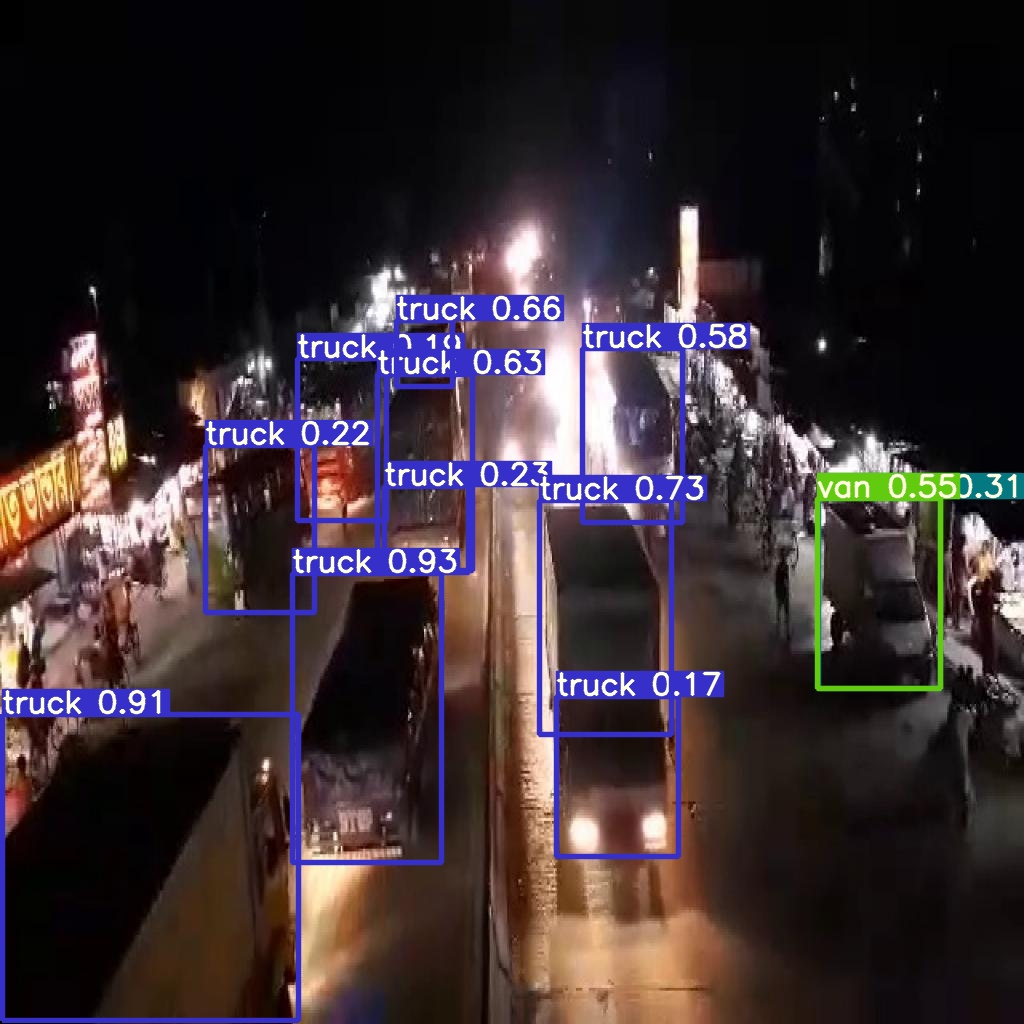
\includegraphics[max width=\textwidth]{images/ours/3 (1).jpg}
   \caption[Sample Inference of Vehicles 6]{ Sample inference vehicles at night}
    \label{fig:inference34567}
\end{figure}

In~\ref{fig:inference34567} our model detects vehicles during night. We can easily see that it can detect trucks with very high accuracy but fails to detect rickshaws and buses which have a high accuracy rate during day time. Because our dataset lacks images of night time. But we have many images of trucks during both night and day. That is why we can detect trucks and other related classes in night time accurately.

\newpage

\begin{figure}[ht]
    \centering
    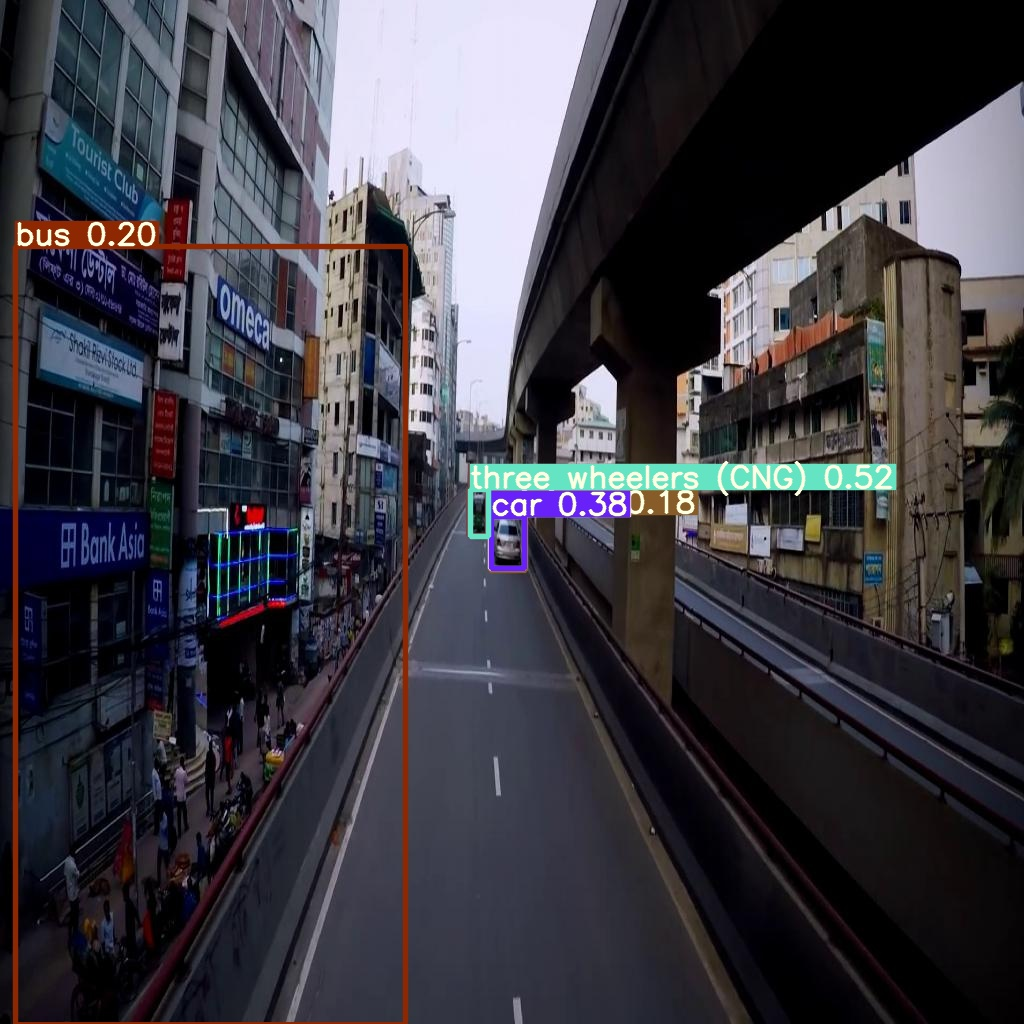
\includegraphics[max width=\textwidth]{images/ours/3 (3).jpg}
   \caption[Sample Inference of Vehicles 7]{Sample inference of false positive during dusk}
    \label{fig:inference346}
\end{figure}

In~\ref{fig:inference346} we can see our model detecting small vehicle objects with good accuracy but it detects sides of road block building as bus because of low light and having similarity with edges of bus. It is a blunder mistake but it has very low confidence with this false positive result.
\newpage


